\chapter{Business Model for the Microsoft Kinect Based Exercise Game}
The product Cyberlab is going to develop and sell is a Microsoft Kinect based exercise game for people over 65 years old. Cyberlab has to find a way to create and deliver the game and capture value from the game. This can be described be the help of a business model, as suggested by Osterwalder \cite{osterwalder}. In this chapter we will provide a detailed description of a business model for the exergame. As a framework for this description, we will use Osterwalder's Business Model Ontology, as described in chapter 4. The interviews conducted will lie the foundation for the business model, as well as our own -and previous research. 

\section{Product}
A product covers all aspects of what a company offers to its customers. The product is composed of value propositions, which are services and values offered to the customer. Cyberlab will develop an exercise game used by physiotherapists in prevention and rehabilitation for elderly. The focus of the exercise game is to improve strength and balance in elderly to prevent fall and injuries. The idea is that this game should have one general workout version directed towards prevention and one customized version used in rehabilitation.
\subsection{Value Proposition}
Value propositions refer to the value a company offers to a specific customer segment. One of the values this product gives to the customer is an opportunity to offer an alternative, fun and motivation training method. The exercise game could be used as a supplement in training programs or as an exercise motivator. A good motivator is a social aspect, which is highly important for elderly, and that there exist games for different interests. The game could also be used as a tool for physiotherapists to make it easier to customize training programs for their patients. Every patient is different, with individual problems and needs, and it is therefore necessary to provide personalized exercise program for each patient. An important value the product has to serve is that the exercise game can set up training programs and be more motivating than a physiotherapist can. To get a consultation hour at a physiotherapist there is often long waiting lists, so it is important for the physiotherapists to be efficient to serve as many patients as possible, without losing quality in the work done. By using this exercise game it is possible to ease the physiotherapists’ workload. The ability of this game is that it can serve more than one player at the same time, which means that a physiotherapist can consult and exercise with more patients in one hour than a physiotherapist can manage without the exercise game. This would be a helpful in the work of shortening the long waiting lists.
\section{Customer Interface}
In this section we will describe how Cyberlab can create value to the customers. Who are the customers, how will they establish contact with them and how will they maintain customer relationship after sales.
\subsection{Customer Segments}
In general, a company generates value for a specific customer segment. The target customers for Cyberlab in this business model are public and private physiotherapy clinics. These are entities with a very close relationship to elderly, and a goal for a physiotherapist is to help elderly decrease the risk of falling by using mobility techniques to improve balance and physical strength. In the starting phase we will recommend Cyberlab to focus on public clinics and private clinics with economic support from the government ("driftstilskudd"). Remaining private clinics will at the moment not be considered as a target customer in this business model. These clinics have other decision making processes, different economy aspects and often a more limited customer base compared to public physiotherapy clinics. With no support from the government these clinics might have a more restricted economy, which complicates purchase of new products. As mentioned, private clinics do not have the same access to customers as public clinics. One reason for this is that customers who consult private clinic have to pay for the therapy session themselves. Elderly may not have that kind of money or willingness to pay for a therapy session at a private physiotherapy clinic (REFERERE til mail med Nina?). Since elderly are the end user of this product, and this group will be challenging to reach through private institutes, we will recommend Cyberlab to not focus on this entity. \\ \\
The customer will not always be the end user, and it is important to recognize and pay attention to this difference. A satisfied end user is important for the customer, although they are not the same person. For this business model physiotherapy clinics will be Cyberlab's customers, while elderly are the end users. For a physiotherapy clinic, elderly will be both the customer and the end user. (Komme med et eksempel?). In the beginning we were thinking about elderly as a target customer segment for Cyberlab as they are the end users of the product, but after working with and studied this business model we experienced that elderly is not the proper target for Cyberlab right now. Some reasons are worth mentioning. Elderly today usually do not have any connection to video games or technology at all. So a developer trying to sell this exercise game by presenting this products value proposition to a person who do not have any knowledge about this area, will be meaningless. The number of technological devices existing today are endless. It will be very difficult for Cyberlab to reach directly out to this customer segment. A solution for Cyberlab to reach their end users is to use someone elderly trusts and rely on. As many others, elderly relies on authorities. Physiotherapists are an example of that kind of authority, so if a physiotherapist tells an elderly that "this product will be good for you", they will most likely believe them. (Legge til eldrehjem, at eldre kan bli brukergruppe senere?) \\ \\ 
\subsection{Channels}
This subsection about distribution channels describes how Cyberlab should deliver and market their value propositions to the customers. We will describe this by going through the five channel phases.
\begin{figure}
\label{fig:Channels}
\begin{center}
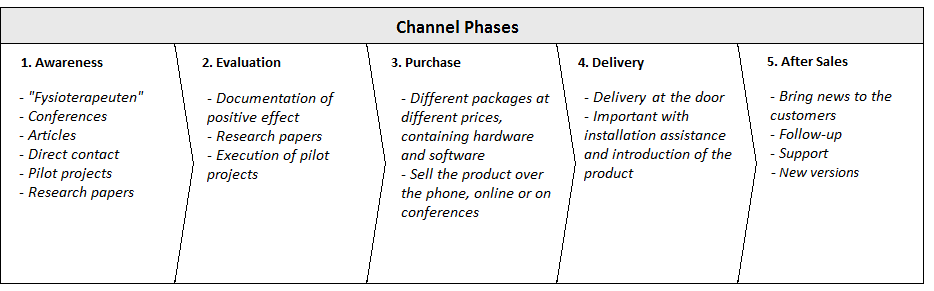
\includegraphics[angle=90,scale=0.7]{channels}
\caption[Channels]{The 5 Channel Phases [modified from \cite{osterwalder}\cite{osterwalderthesis}]}
\end{center}
\end{figure}

\emph{Awareness:} \\ 
We will look into how Cyberlab can raise awareness about the product and how they can get their customers attention.  "Fysioterapeuten" is a magazine targeting physiotherapists in Norway. It is published by \ac{nff} and distributed out to the whole country. "Fysioterapeuten" contains mostly scientific papers, and the idea is that this magazine shall contribute to evolvement of the physiotherapy profession according to the society and populations need. This magazine is read by 9 000 physiotherapists around the country, and articles printed here are seen as scientific and are therefore taken seriously. If Cyberlab could get an article or ad in “Fysioterapeuten” it will contribute to great exposure of the exercise game.  Printing research papers and articles about the exercise game in other credible magazines or newspapers could also get physiotherapists attention.  Taking direct contact with target customers is also a possible solution. This could be done on conferences related to the subject of e.g. technology and health or by visiting physiotherapy clinics. Cyberlab could get the opportunity to present the products and show direct interest in establishing a customer relationship. Physiotherapists see it as very relevant to try a product for an amount of time before they decide to buy. By taking direct contact Cyberlab can introduce a pilot project to the customer, which means testing the product for free in e.g. 6 months. Through conferences, magazines or just word of mouth one can also get an impression of which products that are popular right now. The popularity mark might attract some customers. Physiotherapists working at private clinics do not have the same access to customers as public clinics have, so they might chose to buy a popular product to attract new and more customers. (vet ikke om dette passer under her..)\\ \\ 
(Nav- hjelpemiddelsentralen)\\ \\
\emph{Evaluation:}\\
Physiotherapists points out two very important aspects in evaluating a product. These two are; documented effect of the product and own experience by testing the product. If a physiotherapist should even think about trying the product, it is necessary to provide research papers or statistics that shows positive effect in this kind of games. Documentation will give them a security in the choice of buying the product. (Merkelig setning??) Other physiotherapists providing positive feedback after trying the game also contributes to this security. Another part of the evaluation is by letting physiotherapist be part of pilot projects for a period of time. Then they will have the possibility to test, experience and evaluate the product themselves.\\ \\
\emph{Purchase:} \\
Most physiotherapists have already established connections with suppliers. Ordering and buying products are usually done online, but it can also be by phone or when interesting products are discovered on conferences. Going to the store to buy products is very unusual. But what will physiotherapists buy from Cyberlab? To play this game you need Microsoft Kinect sensor and the exercise game. It is unreasonable to think that a physiotherapist already owns a Kinect sensor, so the best strategy for Cyberlab would be to sell packages containing both hardware and software.  Packages should include various agreements with appropriate pricing. Some examples are selling the package with or without installation assistance and introduction to the product, or by selling a license agreement and "give away" the package for free.\\ \\
\emph{Delivery:}\\
When buying a new product, especially technical products, there is a need for introduction to the product and maybe also installation assistance. Feedback from interviews with physiotherapists shows the huge importance of start-up help. With much to do at work already, physiotherapists do not have time to pick up deliveries at the postal office, or to setup and learn a new product all by themselves. Buying, receiving, installing and learning should not be difficult or time consuming. The product should be delivered at the door, by someone who can install the product and teach the physiotherapists how to use it.\\ \\
\emph{After sales:}\\
When taking a new product in to use, it is important for physiotherapist to have the possibility to come with feedback. Therefore, Cyberlab should have some kind of support that can take these feedbacks into consideration. Feedbacks can be comments on direct errors or directions on how to make the exercise game more suitable for its use. Cyberlab should follow their customer in the process of learning, and they should inform them of new features and improvements.  
\subsection{Customer Relationships}
Customer relationship is an important part of the customer experience, and it describes what kind of relationship the company establishes with the customers. Support, follow-up and feedback handling are some aspects in establishing customer relationship. Cyberlab has to be available when the customers has problems and needs help. When using a new product one may discover errors or find the product not suitable for its use, so many physiotherapists have an eager to provide feedback on this. Cyberlab should handle these feedbacks, fix errors as soon as possible and take comments on improvements into consideration. Using feedback to make a better product shows customers that Cyberlab takes their comments seriously.  In addition, the customers will hopefully get a more suitable product. The maintenance of a direct and personal contact with the customer shows interest in the use and the experience of the product. All this can contribute to a good customer relationship. Cyberlab should also give their customers a heads ups on updates, new features or products.
\section{Infrastructure Management}
This section is about how Cyberlab creates value. What resources needed and what activities that have to be preformed are described here, as well as if they will get them in-house or from a partner. 

\subsection{Key Resources}

In this section we will describe all the resources needed to make the business model work. The resources are divided into 4 different types, described in table \ref{tab:Resources}.
\newpage

\begin{table}
\centering
    \begin{tabular}{|l|l|}
        \hline
       \textbf{Type of Resource} & \textbf{Resource}  \\ \hline
       \emph{Intellectual} & Insight and experience with fall problematic in elderly \\ \cline{2-2}
        & Programming skills \\ \cline{2-2}
	 	& Creativity \\ \hline
	   \emph{Physical} & Premises \\ \cline{2-2}
	   	& Equipments, i.e. desks and computers \\ \cline{2-2}
	   	& Microsoft Kinect HW \\ \cline{2-2}
	   	& Working Environment \\ \cline{2-2}
	   	& Internet Connections \\ \hline
	   \emph{Human} & System Developers, i.e. programmers and interaction designers \\ \cline{2-2}
	   	& Administration, i.e. marketers, customer related tasks \\ \cline{2-2}
	   	& Support Person(s) \\ \hline
	   \emph{Financial} & The European Union \\
        \hline
    \end{tabular}
    \caption[Resources]{Different types of resources}
    \label{tab:Resources}
\end{table} 
\emph{Intellectual} \\ The developers needs insight and knowledge about different exercises that will strengthen muscles and improve balance in elderly. A thorough background study and research have to be conducted to acquire this knowledge. When they have enough knowledge to form the foundation of an exercise program, they can start to get creative. Creativity is needed to make the game entertaining and easy to understand and conduct. In addition, good programming competencies is needed to develop the game. To make it as cost-efficient as possible, an experienced team should be put together. \\ \\
\emph{Physical} \\ To be able to conduct this project, the team need premises with everything that comes with it, like desks, chairs, computer, internet connection, light etc. Cyberlab is an already established business, so we can assume they already have these premises and equipments established. For this project, they will need specific hardware. The hardware consists of a server for storing and running the game, a Kinect sensor, projector and a screen. In addition an environment where the game can be developed is needed. \\ \\
\emph{Human} \\ Programming skills and creativity are already described above as intellectual resources. So system developers and interaction designers are needed. An administration is needed for marketing, customer related tasks and resource management. When the game is finished it needs to be operated and maintained. These tasks can be done by one or more of the system developers. \\ \\
\emph{Finance} \\ This project is financed by the European Union. 
\subsection{Key Activities}
The game can be described as a Value Chain, which means transforming inputs to a final product. From the knowledge and experience they have acquired the company wants to make a product as good and price-competitive so that their customers would choose their product instead of a product with similar value. A description of the different stages in the value chain is depicted in figure \ref{fig:ValueChainCase}. In some way it can also be thought of as kind of a Value Shop, because they are in some way solving a problem for a specific customer segment. To do this, they will work in an iterative way, where they will have to test and evaluate the game during the development process. The users have to be involved during the development. 
Activities that need to be done include research, development, testing, maintenance and updates, support, marketing and administrative tasks. 

\begin{figure}
\label{fig:ValueChainCase}
\begin{center}
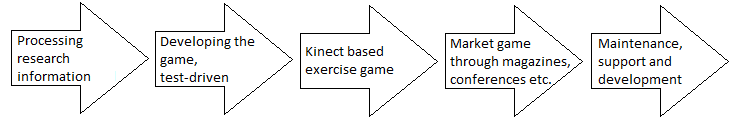
\includegraphics[scale=0.7]{valuechaincase}
\caption[Value Chain for the Kinect Based Exercise Game]{Value chain for the Kinect based exercise game [modified from \cite{osterwalderthesis}]}
\end{center}
\end{figure}
\newpage

\subsection{Key Partnerships}
The main partner in this project is the partnership with Microsoft. There are several reasons for this. First of all, they need the approvement that they are allowed to develop games compatible with their sensor, and second, they need Microsoft hardware and development environment. They will also have to form an agreement with Microsoft on how they can sell the product. \\ \\ As mentioned in the introduction, this project is a collaboration between many different entities, where Norut, a national research group, is one of them. Their job in this project is to provide Cyberlab with research. \\ \\ Physiotherapists are their customer segment, but they can also serve as a partner. Becoming partners with different clinics, will make the the marketing and selling easier, because then the actual customer believes in it. \\ \\ If professionals, physiotherapists believes in this, then the government should believe in it. Getting this game into a medical program financed by the government will make this game very credible for the end user. The government could then provide the game to hospitals, care centers, physiotherapy clinics, training groups, and for special cases, when the elderly for example need the game in their own house. \\ \\ This game can fit well into "Samhandlingsreformen", described in chapter 5. We see this games potential as a too for "everyday rehabilitation" (See chapter 5). This require a collaboration between Cyberlab, physiotherapists and the government. Becoming partners with the Norwegian government will first require that the physiotherapists believes in it, so they will first have to join the team. But it is not a requirement that physiotherapists become a partner. However, some kind of collaboration has to be established with the physiotherapists, since they serve as the professionals. This will typically happen in the research, - development -and testing phase.  \\ \\ Having the Norwegian government as a partner will solve some of the financial issues. Most hospitals, physiotherapy clinics and training groups are managed and financed by the government. With them believing in the game and including it as a helping tool that will prolong and improve elderly's life it will be easier to hit the target users. 
\section{Financial Aspects}
In this section all the outgoing and incoming money will be described. All the previous blocks described are contributing to a cost or an income. We will try to provide an as realistic and detailed estimate of both costs and income. For convenience we will only take the Norwegian market into account. (Si noe om v{å}re forutsetninger for {å} kunne beskrive kostnader og inntekter)
\subsection{Revenue Streams}
The revenue stream describes how the company can earn money, and for Cyberlab this involves selling a product package consisting of the Microsoft Kinect sensor and the exercise game. There are various ways to sell this product, and we will present two solutions.\\ \\
Before pricing the product it is necessary to observe today's market with possible target customers, prices on existing games and physiotherapy tools, and the potential demand for this product. Demand will depend on the documentation of the product and popularity within the physiotherapy community, as well as the product price. Calculating an exact demand for this product is almost impossible due to the lack of existing games in the same genre for this purpose, and also since the game Cyberlab are going to sell do not exist yet. In this section we will assume that the exercise game has been developed, tested and that it has received a great amount of positive feedback. Physiotherapists in Trondheim has started to use the exercise game, and it is being appreciated at the same level as other tool used at the clinic. \\ \\
Pricing this product depends on existing games and tools, and development cost in hope of achieving a non-negative profit for Cyberlab. We can start by looking at existing products. Cyberlab's exercise game falls under two definitions, a video game and a tool used in physiotherapy for training and rehabilitation. The video game market today exist of a huge amount of various games. They are mostly in an affordable price range, where e.g. Nintendo Wii games are priced between 99 - 249 NOK and Xbox Kinect games are priced between 199 - 499 NOK. Physiotherapy tools has more variation in price range as the definition of this tools are quite wide. Prices can vary from a fixed price of 75 NOK for a stretch pulley (http://www.ilenfysioterapi.no/priser/)  to 11 000 NOK per month for shockwave therapy leasing (see appendix “Intervju med Nina”). As we will present later, a package consisting of hardware and Cyberlab’s exercise game will have a much higher price than other video games on the market. Trying to sell the exercise game for more than the already existing ones will be difficult, so it is therefore highly important for Cyberlab to promote their product as more than just a regular game to justify the price difference. This should be done by emphasizing the products value propositions, which relates the product more to physiotherapy equipment than "just" a video game. \\ \\
Cyberlab’s market potential, which is also important for setting a suitable price, can be roughly calculated by looking at the number of public and private physiotherapy clinics with support from the government, from now on referred to as physiotherapy clinics or just clinics. We looked at four municipalities in Norway; Oslo, Trondheim, Fredrikstad and T{ø}nsberg, where we for each found the number of clinics and compared that number to the population in each municipality. The average ratio we got describe inhabitants per clinic in Norway. Multiplying this with the total population in Norway gave us an approximation of physiotherapy clinics suitable for Cyberlab's customer segment. Our calculation (see Appendix blabla for details) shows that Cyberlab has a possible market in approximately 1 200 physiotherapy clinics in Norway. It should be mentioned that the market potential can become bigger if Cyberlab takes private physiotherapy clinics without any economic support from the government into consideration. These clinics has shown interest in this product, which makes them potential target customers. Also, after some time, when the product has been on the market for a while, physiotherapists has got the time to work with the product and elderly has used the exercise game with assistance in a safe environment, it might be time for Cyberlab to think about expanding their market and start selling the product to end users, the elderly. This will increase the market potential significantly. The package price for the end user has to become drastically lower, and with a greater market potential Cyberlab will have the opportunity to sell their products to a lower and more affordable price for an elderly. Private clinics and elderly will not be taken into consideration when discussing Cyberlab's revenue stream.\\ \\
It will be natural to assume that Cyberlab, after documenting positive health effect on their product, will experience interest and demand for their exercise game in Trondheim. Because the product is being developed in Trondheim with close relationship to the hospital, scientist and physiotherapists, the word of the game will be spread in sectors related to Cyberlab's target customer segment. A reasonable place to start marketing and selling the product would therefore be in Trondheim. Cyberlab has as mentioned worked with some of the clinics, they would have the possibility to follow the startup phases closely, and they can respond quickly to requested changes or when eventual errors occur. If Cyberlab can establish a customer base in Trondheim consisting of e.g. 10 physiotherapy clinics and the feedback from these clinics are positive, the game’s reputation might spread to other parts of the country. Selling the product to 10 physiotherapy clinics to a suitable price will not provide Cyberlab with any profit, so it’s absolutely necessary to reach out to other cities and municipalities. (SI noe om at ordet sprer seg lett? Si noe om vanskeligheter ved {å} spre nye produkter?)\\ \\
We will now present two different solution for how Cyberlab can sell their product, with suitable prices for each solution.\\ \\
\begin{figure}
\label{fig:RevenueStreamPrice}
\begin{center}
\includegraphics[scale=0.8]{revenuestreamprice}
\caption[Price example]{The lowest possible package price Cyberlab can have, provided that they sell the max amount of  copies - 1 200 units, is 2650 NOK}
\end{center}
\end{figure}
\emph{Solution 1 - Fixed price}\\ 
The first solution is to sell the product as a package consisting of both software and hardware to a fixed price. Included in this package is delivery, installation assistance, and introduction to the product. We believe it is necessary  to sell the product included in a total package for several reasons. Assuming that physiotherapy clinics already possesses needed equipment as a Kinect sensor, projector or screens big enough is unreasonable to assume. Neither is it reasonable to believe that physiotherapists will buy software from Cyberlab and then walk to the store to buy rest of the equipment. In the package we have also included installation help and introduction, which we have experienced as important for physiotherapists. For this type of technology equipment it is useful to give an introduction to the product. We can not expect that physiotherapists have the time to teach themselves how the products work. This could result in physiotherapists buying the product and ending up never using it because of the lack of information. \\ \\
The package price will cover wages for the hours of installation and introduction, hardware, and other cost connected to development, investment and marketing of the product. For Cyberlab, total cost is approximately 3 170 000 NOK (see Appendix KinesRegneark). This number does not include purchase of hardware in the packages or wages for installation and introduction. In this section we will not take wages for installation and introduction into account, as it is very difficult for us to calculate all costs connected to this. We will now look at different price proposals. If we assume that Cyberlab has the possibility to sell their product to all of the 1 200 physiotherapy clinics in Norway, they could have a price as low as 2 650 NOK, see Figure \ref{fig:RevenueStreamQuantity}, without gaining negative profit. However, it is very risky, almost unreasonable, to assume that Cyberlab could reach out to all target customers. Figure \ref{fig:RevenueStreamPrice} shows three income lines related to three different prices. With a price of 6 000 NOK Cyberlab needs to sell at least 529 units to achieve non-negative profit, but with a price of 10 000 NOK they only has to sell 317 units. How many units Cyberlab has potential to sell and what price customers are willing to pay depends on demand, which we have mentioned is difficult to measure. A maybe more reasonable sales number would be to cover a third of the possible market share, which is about 400 units. (Si noe om: dette pga av usikkerhet rundt spillet, det er nytt. Ikke alle klinikker har behov. Konservativ gjeng. Ingen lignende teknologi. Ikke s{å} kjent med teknologi). Pricing these units at 8 000 NOK will give Cyberlab some profit. (Hvordan skal jeg begrunne hvilken pris jeg b{ø}r ta? Kanskje se p{å} noen andre utstyr fysioterapeuter bruker og sammenligne pris). (Se p{å} kommunens budsjett til fysioterapeuter). However, to also include hardware price in the final package price, the customer will have to pay significantly more for the product. The Kinect sensor, projector and screen costs approximately 5 140 NOK, which means  that the final package price will end up at 13 140 NOK if Cyberlab choose to price their exercise game at 8 000 NOK.\\ \\
\begin{figure}
\label{fig:RevenueStreamQuantity}
\begin{center}
\includegraphics[scale=0.7]{revenuestreamquantity}
\caption[Quantity examples]{Total cost and three revenue lines related to three price examples; 6 000 NOK per unit, 8 000 NOK per unit and 10 000 NOK per unit, shows minimum number of units Cyberlab has to sell to achieve a non-negative profit}
\end{center}
\end{figure}
\emph{Solution 2 - License agreement}\\
The second solution is to sell the same package as in the first solution, where the package here is implemented in a license agreement. Customers will pay a low start price for the package, and a certain amount of money for each time they use the product. This low start price will not alone cover all of Cyberlab’s total costs, even if they sell to all their potential customers, so it depends on customers using the product. As in the first solution, Installation and introduction is also here included in the package, but it will not be taken into consideration when we describe package price proposals. \\ \\
We will start by making an estimation of how much this exercise game potentially will be used. Usually, a physiotherapist works approximately 8 hours a day, which includes 30 minutes lunch. Not every patient visiting the physiotherapy clinic during a regular day falls under the category “elderly”, and not every elderly visiting the clinic has the need or wants to use this exercise game. We roughly estimate that the exercise game will be used approximately 2 hours a day. A physiotherapist works 47 weeks a year, assuming they have 5 weeks of vacation, and this adds up to 470 hours a year where the exercise game will be used.\\ \\
A proposal for a suitable price for this license agreement is a startup price of 2 000 NOK for the package and a price of 50 NOK (Begrunne denne prisen med total pris for en time, hvor mye de sparer p{å} effektivitet/ha flere i samme time) for each hour physiotherapists use the exercise game. During a year this will add up to 25 500 NOK. In the first solution, the price for hardware was added on top of this total price, but here this is included in the license agreement. Therefore, since Cyberlab’s total costs is measured without consideration of the hardware price we subtract this price from the estimated revenue. So, for each customer purchasing this license agreement, Cyberlab will have an estimated revenue stream of approximately 20 000 NOK. We observe that Cyberlab in this case only need to sell approximately 160 units to make a profit. The income increases much more in this license agreement example than in the fixed price example. Where we in the first example showed that Cyberlab barely achieved profit by selling 400 units, they can with this license agreement sell the same amount of units to a profit of 4 830 000 NOK (See Appendix blabla). \\ \\	
\begin{figure}
\label{fig:RevenueStreamLicense}
\begin{center}
\includegraphics[scale=0.8]{revenuestreamlicense}
\caption[License example]{Profit when using license agreement(blabla}
\end{center}
\end{figure}
We can conclude that selling a license agreement is the best solution for Cyberlab. The possibility of gaining a non-negative profit is higher, and the profit has the potential of becoming much higher than with a fixed price solution. We can conclude that selling a license agreement is the best solution for Cyberlab. The possibility of gaining a non-negative profit is higher, and the profit has the potential of becoming much higher than with a fixed price solution. There will be some risk related to this license agreement. As mentioned, the low startup price for the license agreement is not alone enough to cover all of Cyberlabs costs, so even if Cyberlab manage to cover the whole market they will experience a huge economic loss if no one use the product. Since the idea is that the startup price of 2 000 NOK should cover Cyberlabs costs and the hardware price, we can easily understand that this will lead to a major loss. If we predict that Cyberlab sell the likely amount of 400 units, and no of the customers use the product, they will have a negative profit of - 4 570 000 NOK. However, if all of the 400 customers use the exercise game, only one hour a day for a year will be enough for Cyberlab to gain non-negative profit. Expected life time for a game like this is approximately 5 years, so Cyberlab is actually only dependent on customers using the game one hour a week to gain non-negative profit, which is very likely! (see Appendix blabla2) \\ \\   
For the customers point of view a license agreement will appear more appealing than a fixed package price because of the low startup price (trekke inn noe psykologisk rundt kj{ø}psprosesser). Customers observe that the product price is higher than other existing video games on the market, but they also know what value propositions this exercise game holds, which justify the price difference. They also have information about prices on equipment used at physiotherapy clinics, which makes Cyberlab’s license agreement affordable. Customers also have other reasons for why they prefer this solution. One example is “Ilen Fysioterapi og Idrett”, a private physiotherapy clinic with no economic support from the government, which sees a security in the possibility of buying the product with a license agreement (Se Appendix “intervju med Nina”). The startup price is manageable, and they can control additional costs themselves after how much they want to use the equipment. Private physiotherapists might not have the same financial resources as local institutes, so the idea of paying according to how much they use the product is appealing. 

\subsection{Cost Structure}
Cost structure takes into account all elements that generates costs specific to this game. Cyberlab is an already established business and we can therefore assume that there are not any additional costs associated with premises and some of the "regular" equipments (e.g. desks, chairs, computers etc.). First we distinguish between fixed and variable costs, investment costs and ongoing costs. Variable costs are associated with demand. In this case it is hard to say anything about the demand. Therefore we do not have sufficient knowledge to say anything about the variable costs. For this game, the variable costs will be salaries associated with support, maintenance, marketing and sales. However, since we are dealing with a market which is very hard to analyse with respect to demand, we will make a prediction on how much work is required for each of this tasks, for each year of the game's lifetime. Thus, in our analysis, all the costs will look like fixed costs.  \\ \\
In this case fixed costs are associated with salaries to all the involved workers on this project. The reason why we define these as fixed costs is because the employers are assigned this project for a fixed period of time (this especially accounts for the employers in the developing-phase, but we will also assume this for all other involved employers). This includes project manager, developers, interaction designers, support, marketers and salesperson. There are additional costs associated to having an employee, explained shortly. The investment costs associated to this project is the hardware and software needed to develop the game. This includes specific hardware and a \ac{sdk} for the sensor. The commercial price for the Kinect sensor is 1790 NOK \cite{pricekinect}, and the \ac{sdk} for the sensor is free. In addition they should have a screen for testing purposes. The screen should be of significant size, so we suggest they invest in a projector and 90" projector screen, which should be sufficient for its purpose. We found that the cost of an average screen lies around 895 NOK and 2449 NOK for a projector \cite{priceprojector}\cite{pricescreen}. \\ \\
Cyberlab has estimated that for the developing of this game they need a \ac{fte} = 1.0, meaning that the workload is equivalent to one person working full time for a year. We assume that this will cover development, testing and administrative tasks. In addition to that, Norut who provides research has also assigned a \ac{fte} = 1.0. How many people assigned to the project is unknown and also irrelevant for the cost prediction, (assuming each employee has the same salary). We have done a rough estimate on how much the cost of having \ac{fte} = 1 in the private sector is. From \cite{tekna} we found statistics of salary in the private sector in Norway. Assuming that the "average" employer on this project graduated in the end of the 90's, we look at an average gross salary of approximately 730 000 NOK a year. From this we can calculate the average cost of a \ac{fte} = 1.0, based on \cite{altinn}, see Table \ref{tab:costofFTE}, which will be 1 003 349 NOK. We did the same calculations for researchers in the government controlled sector and for marketers in the private sector. They both ended up on a cost of 715 577. See appendix for calculations. \\ \\

\begin{table}
\centering
    \begin{tabular}{|l|l|l|r|}
        \hline
       1&Gross Salary & & 730 000 NOK \\ \hline
       2&Holiday Pay & 12.1\% of 1  & 88 330 NOK \\ \hline
	   3&Employee Fee & 14.1\% of 1+2  & 115 385 NOK \\ \hline
	   4&Pension Costs & 8.0 \% of 1 & 58 400 NOK\\ \hline
	   5&Employee Fee of Pension Costs & 14.1\% of 4 & 8 234 NOK \\ \hline
	   6&Insurance & & 2 000 NOK \\ \hline
	   7&Mobile and Internet & & 1 000 NOK \\ \hline
	   & \textbf{SUM} & & \textbf{1 003 349 NOK} \\
	    \hline
    \end{tabular}
    \caption[Cost of FTE = 1]{The cost of FTE = 1 in the private sector (for Cyberlab}
    \label{tab:costofFTE}
\end{table} 
We will now look as some ongoing costs on a per year basis. The game has to be operated on a server. This can be on a local server located in Cyberlab’s office, a server located at one of the physiotherapy clinics or on a cloud hosted server. The size of a Kinect game varies a lot, depending on quality, colors, how many levels etc. What we do know is that the game itself will be of fixed size. The dynamic part of the space needed on the server is associated with how many customer profiles it needs to store. This is a hard task to answer, but we assume that the user profiles do not take up that much space, and that Cyberlab can make it with a small server with fixed space. At this stage it is also hard to make an exact assumption on how big the game will become, but from already existing Kinect games, we can assume that the size will not be bigger that 10 GB. From Gogrid Servers \cite{priceserver} we found a small server with storage space of 25 GB. We believe this will be sufficient for Cyberspace's purpose. There is also reasonable to believe that Cyberlab has some space available on their servers. However, if they would have to rent this kind of server space, we are looking at an annual price of \$181.25 which is is roughly 1 087 NOK (with a currency of \$1 = 6 NOK).\\ \\
With new software and technology there will always be some errors and bugs after the product or service is delivered. We can assume that the first six months are the most critical months, and will require a \ac{fte} = 1/5. The remaining life time will only need support for some minor problems that might appear (e.g. customer service, operating the server). We assume this period will require a \ac{fte} = 1/10. This is very hard predictable numbers, because this may vary over time. However, our predicted numbers are reasonable as "average" numbers, taking unexpected events into account. With the rapid evolution of technology, we believe that Cyberlab can offer this game for five years after its release. After, or even during, these years, they will probably have to start making new versions, even for new types of technology. (FINN KILDE PÅ DETTE) We do not take the development of new versions into account in our calculation, and we will set the lifetime of this game to be 5 years. \\ \\
Marketing is one of the most important part of selling a product or service. This is especially important in the first year of the games life time. The cost of marketing is difficult to analyse because it depends on how long it will take to acquire customers. A new product or services need to acquire customers quickly, and therefore more resources need to be put into the marketing tasks. We can look at the exercise game as a niche product that is targeting a specific customer segment. Thus, the marketing task needs to be customized for this specific customer segment. When a critical mass (the number of customers needed to survive economically in the market) is reached the market will somehow be self-supported \cite{informationrules}. We believe that after this critical phase, the marketing costs will be rather low and close to constant. We assume that the first year right before, during and after the release, the marketing task will contribute to a \ac{fte} = 1/2. After being on the market for one year, the customer base should have reached critical mass.  We believe that in this type of community (the physiotherapist community), words spread fast. If someone starts using a product that is proven good, it will soon appear in magazines and by word of mouth, resulting in the interest from more. Even after critical mass is reached, there will still be some marketing related tasks (e.g. keep up with the market, look for new customer segments), so we suggest that the marketing tasks should contribute to a \ac{fte} = 1/5 after the first year. With this low workload, Cyberlab should consider to hire a marketing consultant in stead of having a permanent employee. (Mulig de har en egne markeds- og salgsansatte) FINNE NOEN TALL PÅ Å LEIE MARKEDSFORER.\\ \\
As mentioned we suggest that Cyberlab should run pilot projects to document the effect of the game. This will also serve as a very effective way of marketing the game. We suggest that the pilot project should be carried out in two different clinics in Trondheim for convenience, and that it should run for six month. The effect should be documented during the project and after. This documentation should be published in scientific articles and distributed to physiotherapists. (Lurer på om også offentlige klinikker må ha penger for dette? det er vel de som skal dokumentere effekt osv. Vil jo gi de ekstra arbeid.). We assume that the development of the game will take about six months, so the first year will contain the development phase and the pilot project. The pilot project will most likely provide Cyberlab with valueable feedback on the game, where they can both test the usability in a real environment as well as discover bugs and errors. This will require close monitoring from Cyberlab, so we suggest that this will require a \ac{fte} = 1/5 for this six months (This equals \ac{fte} = 1/10 seen in a whole year). Spending six months on the initial developing and six months on the pilot project, means that Cyberlab is looking at a whole year without revenue. \\ \\
The exergame will be sold with as a package with all the hardware needed to the customer. This makes it more convenient for the customer and easier to sell. It is not reasonable to believe that Cyberlab will earn money on the hardware. They will need to make an agreement with Microsoft to buy the Kinect sensor and sell it further to the same price. The same applies for projector, screens, and Windows machines. This means that Cyberlab will need to have the liquidity to be able to buy a set of hardware that they later will sell to their customers. We suggest that they should have some hardware in stock for quick delivery. This means that we need to anticipate how many customers will buy the game every year. We believe that it is not unrealistic to look at the S-curve for how much of the market they will take year for year. In the first year they will only take a small part of the market, but as soon as the game gets attention from the rest of the market, it will spin of pretty fast, before it will slow down again when most of the market is saturated. BLIR DET FEIL Å TENKE SLIK?  \\ \\
From the interviews conducted we found that it was desirable with installation and introductory help when buying a technical equipment. This is a complicated task for Cyberlab when we look at every physiotherapy clinic as their customer segment. It is not realistic that one representative from Cyberlab will travel to the other side of the country as soon as an clinic order the game. In the first year, we suggest that Cyberlab focus on delivering the game to clinics in Trondheim. Selling the game in only Trondheim to an acceptable price, will not make profit. We believe that Cyberlab is looking at some years before they will make profit. The physiotherapy community is small and they have a lot of similarities. By the time this game has become well-known in Trondheim, the game has probably got attention from clinics in other cities as well. We suggest that Cyberlab hire some of the physiotherapists that are already using the game to present it on conferences and learn other physiotherapist how to use it. In this way, the game will be both more believable to other physiotherapists, as well as Cyberlab do not need to do the hazel with travel around promoting their game. There is still some costs associated to this. HER TRENGER VI LITT TILBAKEMELDING..\\ \\
Taking all the described costs into account, the project with six years of lifetime (including development and the pilot project) will have a total cost of 3 168 773 NOK. See appendix for calculation (Ikke der ennå). 